\section{Finding 5 - Path Traversal on Apache Server}
%center under chapter title a one row table with 6 coloumns and no borders
\vspace*{-0,3cm}
\begin{center}
    \begin{tabular}{c c c c}
        \textbf{Classification:} & Information Disclosure & \textbf{Severity:} & \textbf{\textcolor{red}{High}}  
        \end{tabular}
\end{center}

\vspace*{-0,8cm}
\begin{center}
    \begin{tabular}{c c}
        \textbf{CVE:} &
    \end{tabular}
\end{center}

On the Apache Server of the \ac{DUT} (port 80) it is possible to access directories via path traversal. By adding the path ”/home/...” to the URL it is possible to see directories which seem to be users of the \ac{DUT}.
The directories are empty.

\subsection*{Finding Impact}
The Impact of this finding is an severe Information Disclosure. Attackers could try to guess passwords for the found users and eventually gain access to the \ac{DUT}.

\subsection*{Finding Details}
A way to find the path is to use a nmap scan with the ”http-enum” script:
\begin{lstlisting}[language=bash]
$ nmap -A --script -http-enum 172.16.0.29

PORT STATE SERVICE VERSION
80/top open http Apache httpd 2.4.54 ((Debian))
|_http-server-header: Apache/2.4.54 (Debian)
| http-enum:
|_ /home/:
Potentially interesting directory w/ listing on 
'apache/2.4.54 (debian)'
\end{lstlisting}


To see the directory it is possible to visit the URL in a web browser:
%insert an image but in this subsection*
\begin{figure}[h]
    \centering
    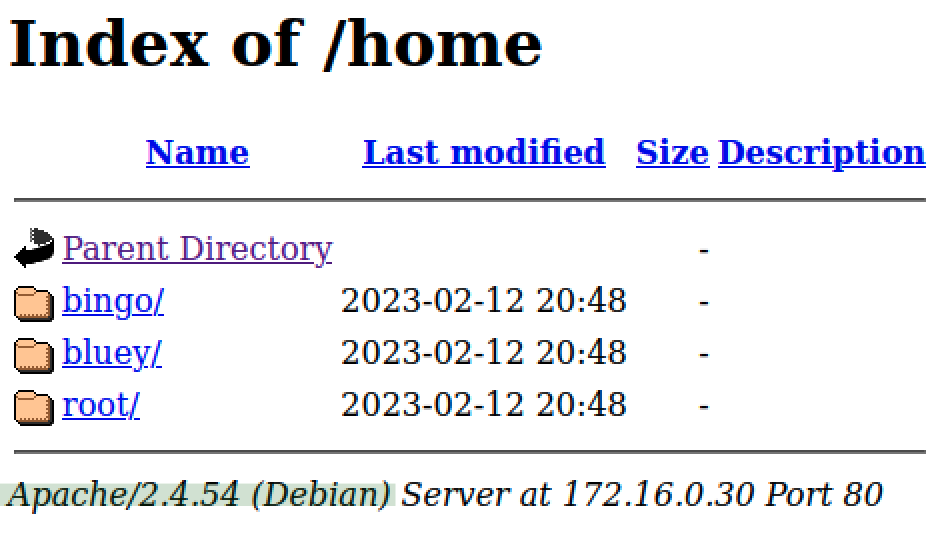
\includegraphics[width=0.8\textwidth]{img/apache-version.png}
    \caption{Path Traversal}
    \label{fig:fin5}
\end{figure}

\subsection*{Evaluation of Results}
\begin{center}
    \begin{tabular}{cccc}
    \textbf{Effort to Fix:} & &\ \textbf{\textcolor{orange}{Medium}}\
    \end{tabular}
\end{center}
The Server should validate the path before accessing it. A possible solution could be to whitelist the allowed paths, which should be accessible. This would prevent accessing directories of the \ac{DUT} which are not intended to be accessed by the user.